
%(BEGIN_QUESTION)
% Copyright 2010, Tony R. Kuphaldt, released under the Creative Commons Attribution License (v 1.0)
% This means you may do almost anything with this work of mine, so long as you give me proper credit

An electrician goes to troubleshoot a three-phase motor starter (``bucket'') that is not functioning.  When the operator presses the ``Start'' switch, the motor refuses to start up.  Thinking that perhaps one of the main fuses is blown, the electrician measures AC voltage across each fuse, measuring 0 volts drop for each one.  Upon seeing this, he declares all three fuses to be good, and that the trouble must lie elsewhere in the circuit (e.g. bad motor, failed contactor, etc.).

$$\includegraphics[width=15.5cm]{i03737x01.eps}$$

Explain what is wrong with the electrician's reasoning, and how it is possible to measure 0 volts across a fuse that is actually blown.

\vskip 20pt \vbox{\hrule \hbox{\strut \vrule{} {\bf Suggestions for Socratic discussion} \vrule} \hrule}

\begin{itemize}
\item{} Identify which fundamental principles of electric circuits apply to each step of your analysis of this circuit.  In other words, be prepared to explain the reason(s) ``why'' for every step of your analysis, rather than merely describing those steps.
\item{} This is an example of a logical fallacy known as {\it illicit conversion}.  A general example of this fallacy goes like this: ``All rabbits are mammals, therefore all mammals are rabbits.''  Explain how the electrician's association of 0 volts with a good fuse is an example of this fallacy.
\end{itemize}

\underbar{file i03737}
%(END_QUESTION)





%(BEGIN_ANSWER)

A measurement of 0 volts {\it may} imply electrical continuity, but it may not.  There are other reasons why one might obtain a 0 volt measurement, such as an open fault isolating the measurement points from power.  If some {\it other} part of the AC line is open (e.g. the contactor being de-energized), even an open fuse will drop 0 volts because it is not the only open in the circuit.

%(END_ANSWER)





%(BEGIN_NOTES)


%INDEX% Troubleshooting review: electric circuits

%(END_NOTES)

